\chapter{Knowledge And Conflict In Relationship}

This chapter follows J. Krishnamurti's San Diego dialogue with Dr. Alan W. Anderson on knowledge and conflict in human relationship, from source material preserved by the Krishnamurti Foundation Trust and curated for this course by LazyingArt LLC through Video2Book. There is no validated blackboard mathematics for this lecture. The mathematical work of the chapter is therefore a disciplined notation of the spoken inquiry: a way of making the sequence of distinctions visible without turning the dialogue into a formal theory.

\section{The Observer As The Past}

Anderson begins by tying the conversation to the previous one. The earlier inquiry had distinguished the living fact that ``the world is me and I am the world'' from the mistake of taking the description for the described. That mistake now focuses the whole discussion on a single term: the observer. If the observer is confused, what is the observer? Can he relate to the observed in a different way?

Krishnamurti does not treat the observer as a neutral inner witness. He identifies it at once with the past. The past is accumulated knowledge, experience, memory, tradition, image, hurt, hope, demand, and conditioned response. Thought is not new, because thought is the response of that accumulated past.

We will use compact editorial notation. It is not notation from the speaker; it is a reading aid for the chapter:
\begin{equation}
\mathrm{Thought}=\mathrm{Past}.
\end{equation}
The next equality is the decisive one:
\begin{equation}
\mathrm{Observer}=\mathrm{Past}.
\end{equation}
Let
\begin{equation}
O:=\mathrm{Observer}.
\end{equation}
Then the opening diagnosis can be written as
\begin{equation}
O=\mathrm{Past}
=\mathrm{Knowledge}+\mathrm{Experience}+\mathrm{Memory}+\mathrm{Image}.
\end{equation}
The plus signs do not mean a literal algebraic sum. They mark the named elements of the spoken structure. The observer is not outside the known. The observer is the known as it looks.

\begin{proposition}
Observation through \(O\) is already divided observation.
\end{proposition}

\begin{proof}
The observer is identified with the past. The past includes memory, image, hurt, hope, tradition, and conditioned response. When such an observer observes, it observes through this background. Therefore it does not observe wholly; it separates itself as observer from what is observed. That separation is already division.
\end{proof}

This is why the word ``I'' becomes important. Anderson asks whether the person who says ``I'' while taking the description for the described is referring to this observer. Krishnamurti answers by identifying the ``I'' with the past:
\begin{equation}
\mathrm{I}=O=\mathrm{Past}.
\end{equation}
The lecture's first movement is now complete. The problem is not merely that the observer has wrong information. The observer is the accumulated movement of the known.

\begin{figure}
\centering
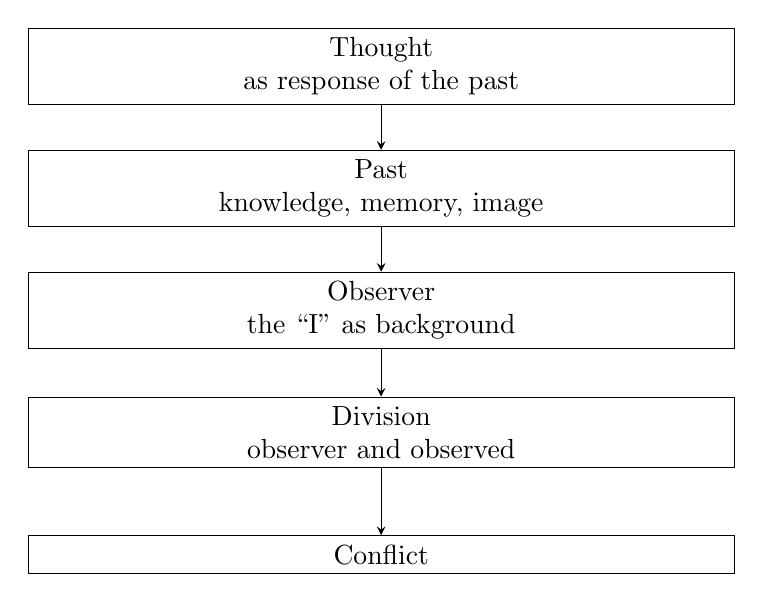
\begin{tikzpicture}[>=stealth]
\node[draw, align=center, text width=0.72\linewidth] (thought) at (0,0) {Thought\\as response of the past};
\node[draw, align=center, text width=0.72\linewidth] (past) at (0,-1.55) {Past\\knowledge, memory, image};
\node[draw, align=center, text width=0.72\linewidth] (observer) at (0,-3.10) {Observer\\the ``I'' as background};
\node[draw, align=center, text width=0.72\linewidth] (division) at (0,-4.65) {Division\\observer and observed};
\node[draw, align=center, text width=0.72\linewidth] (conflict) at (0,-6.20) {Conflict};
\draw[->] (thought) -- (past);
\draw[->] (past) -- (observer);
\draw[->] (observer) -- (division);
\draw[->] (division) -- (conflict);
\end{tikzpicture}
\caption{A transcript-derived reconstruction of the opening chain: thought as past, observer as past, division, and conflict.}
\end{figure}

\section{Freedom From The Known And Creative Action}

Once the observer has been identified with the past, Krishnamurti asks the next question in compressed form: can the mind be free from the known? The motivation is exact. If the known is the repetitive movement of the past, then action born from the known will continue the past, even when it is modified.

This is where the word ``creative'' enters. Krishnamurti pauses over it because it is easily misused. He is not speaking of creative writing, creative pictures, or novelty that wins attention. Novelty can still be modified repetition. Something may look fresh, eccentric, or successful, and yet remain tied to the observer.

The distinction is:
\begin{align}
\mathrm{Novelty} &= \mathrm{Modified\ Repetition},\\
\mathrm{Creative\ Action} &\neq \mathrm{Novelty}.
\end{align}
Creative action, in the sense used here, requires freedom from the known:
\begin{equation}
\mathrm{Freedom\ from\ the\ Known}
\longrightarrow
\mathrm{Possibility\ of\ Creative\ Action}.
\end{equation}

\subsection{Question \& Answer}

\paragraph{Question.}
Does freedom from the known mean rejecting knowledge?

\paragraph{Answer.}
No. Krishnamurti explicitly refuses that reading. Freedom from the known is not the negation of the known. It is the understanding of the known. We have to see where knowledge is necessary, where it functions properly, and where it becomes image, barrier, and division.

The distinction is:
\begin{equation}
\mathrm{Freedom\ from\ the\ Known}
\neq
\mathrm{Negation\ of\ Knowledge}.
\end{equation}
The positive movement is:
\begin{equation}
\mathrm{Understanding\ of\ the\ Known}
\longrightarrow
\mathrm{Intelligence}
\longrightarrow
\mathrm{Freedom}.
\end{equation}

\begin{figure}
\centering
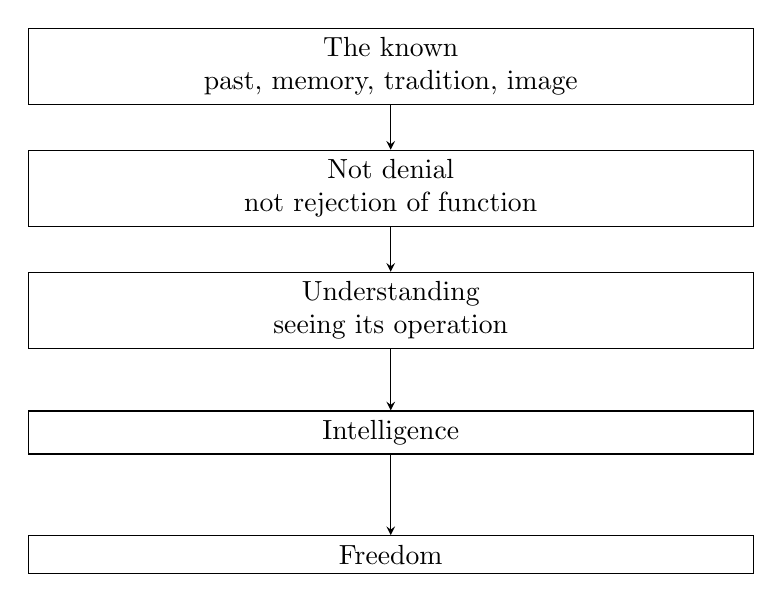
\begin{tikzpicture}[>=stealth]
\node[draw, align=center, text width=0.74\linewidth] (known) at (0,0) {The known\\past, memory, tradition, image};
\node[draw, align=center, text width=0.74\linewidth] (notdeny) at (0,-1.55) {Not denial\\not rejection of function};
\node[draw, align=center, text width=0.74\linewidth] (understand) at (0,-3.10) {Understanding\\seeing its operation};
\node[draw, align=center, text width=0.74\linewidth] (intelligence) at (0,-4.65) {Intelligence};
\node[draw, align=center, text width=0.74\linewidth] (freedom) at (0,-6.20) {Freedom};
\draw[->] (known) -- (notdeny);
\draw[->] (notdeny) -- (understand);
\draw[->] (understand) -- (intelligence);
\draw[->] (intelligence) -- (freedom);
\end{tikzpicture}
\caption{Freedom from the known is reconstructed here as understanding, not rejection.}
\end{figure}

This pause matters. Without it, the chapter would sound as though knowledge itself were the enemy. That is not the lecture's order. First we see that the observer is the known. Then we ask whether the known can be understood so that the mind is not bound by it.

\section{Knowledge As Function, Knowledge As Division}

The dialogue now makes the necessary practical distinction. Knowledge is required for ordinary action. We need knowledge to go home, to speak English, to write a letter, to use tools, to function mechanically. Krishnamurti does not erase that field.

Let
\begin{align}
K_f &:= \mathrm{functional\ knowledge},\\
K_r &:= \mathrm{knowledge\ in\ relationship}.
\end{align}
Then the spoken distinction is:
\begin{equation}
K_f \neq K_r.
\end{equation}
Functional knowledge belongs to practical operation. Knowledge in relationship is knowledge as image, memory, tradition, past experience, and observer. It is the accumulated picture of another human being.

\begin{table}
\centering
\begin{tabular}{p{0.42\linewidth} p{0.42\linewidth}}
\hline
\(K_f\): functional knowledge & \(K_r\): knowledge in relationship \\
\hline
Going home & Image of another person \\
Speaking a language & Memory of hurt or demand \\
Writing a letter & Tradition and conditioning \\
Mechanical operation & Observer acting as the past \\
Necessary for function & Barrier between you and me \\
\hline
\end{tabular}
\caption{The lecture's central distinction between knowledge as function and knowledge as image in relationship.}
\end{table}

The transition is one of the lecture's sharpest turns. Krishnamurti says, in effect: knowledge is necessary to act; now see what happens when that same movement enters relationship. If I use knowledge in my relationship with you, I bring a barrier between us. The knowledge that was necessary in function becomes separating in relationship.

The chain is:
\begin{equation}
K_r
\longrightarrow
\mathrm{Barrier}
\longrightarrow
\mathrm{Division}
\longrightarrow
\mathrm{Conflict}.
\end{equation}
Krishnamurti then widens the scale. The same structure appears between husband and wife, one person and another, India and Pakistan, America and Russia, religious group and religious group. The names vary; the movement of division is the same.

\begin{proposition}
Where knowledge operates as image in relationship, conflict follows.
\end{proposition}

\begin{proof}
Knowledge as image is the past standing between two people. That image functions as a barrier. A barrier produces division. Krishnamurti repeatedly states that where there is division there must be conflict. Therefore knowledge as image in relationship produces conflict.
\end{proof}

This is the chapter's first worked derivation. Written as short steps:
\begin{enumerate}
\item \(K_r\) is knowledge as memory, image, tradition, and past experience.
\item \(K_r\) stands between one human being and another.
\item What stands between divides.
\item Division produces conflict.
\item Therefore \(K_r\) produces conflict in relationship.
\end{enumerate}

\section{Relationship And The Place Of The Observer}

The lecture now arrives at its central repeated question: what place has knowledge in human relationship? More sharply, what place has the observer in human relationship?

This repetition should not be smoothed away. It is the pressure of the inquiry. Relationship is not a side topic. Krishnamurti says there is no life without relationship. Even withdrawal into a monastery is still relationship: relationship to the past, to a rule, to a savior, to an image, to an idea of isolation. Human life is relationship, and society grows out of it.

The repeated question can be written as:
\begin{equation}
\text{What place has } O \text{ in relationship?}
\end{equation}
The tempting answer would be: the observer must learn to relate rightly. Krishnamurti's answer is more severe. The observer is the factor of division. If the observer enters relationship, actual relationship is absent.

\subsection{Question \& Answer}

\paragraph{Question.}
Has the observer any place in human relationship?

\paragraph{Answer.}
No. The moment the observer comes into relationship, division has entered. The observer is the past, the image, the accumulated knowledge of the other. That movement may produce habit, dependence, possession, sexual contact, social arrangement, or mutual use, but it is not actual relationship.

In notation:
\begin{align}
O \in \mathrm{Relationship}
&\longrightarrow \mathrm{Division},\\
\mathrm{Division}
&\longrightarrow \mathrm{No\ Actual\ Relationship}.
\end{align}

This is where Anderson's caution is important. The statement ``the world is me and I am the world'' may itself become an idea. If the mind turns it into a concept and tries to live according to that concept, abstraction has replaced reality. The description has again been taken for the described.

Krishnamurti therefore brings the inquiry back to actuality. In marriage, friendship, family, work, or social life, what is actually going on? If each person is full of private success, money, ambition, envy, hurt, and demand, then the word relationship covers separation. The observer is present, and the observer is the point at which relationship fails.

\begin{figure}
\centering
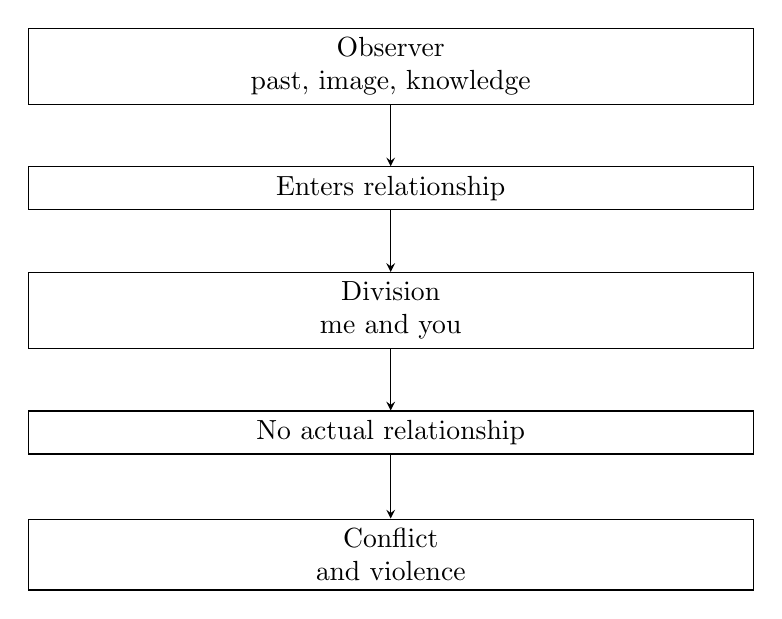
\begin{tikzpicture}[>=stealth]
\node[draw, align=center, text width=0.74\linewidth] (observer) at (0,0) {Observer\\past, image, knowledge};
\node[draw, align=center, text width=0.74\linewidth] (enters) at (0,-1.55) {Enters relationship};
\node[draw, align=center, text width=0.74\linewidth] (division) at (0,-3.10) {Division\\me and you};
\node[draw, align=center, text width=0.74\linewidth] (norel) at (0,-4.65) {No actual relationship};
\node[draw, align=center, text width=0.74\linewidth] (violence) at (0,-6.20) {Conflict\\and violence};
\draw[->] (observer) -- (enters);
\draw[->] (enters) -- (division);
\draw[->] (division) -- (norel);
\draw[->] (norel) -- (violence);
\end{tikzpicture}
\caption{The observer in relationship, reconstructed from the spoken sequence.}
\end{figure}

The movement then turns toward violence. To understand violence, one has to understand division. The example of the child striking the mother is not introduced as a theory of childhood. It is introduced to say: the division was already there. Likewise with national identity and armaments. When one calls oneself American, Russian, Hindu, or something else in opposition to another, division becomes the factor of violence and hatred.

\section{Freedom, Austerity, Order, And Virtue}

After the inquiry into relationship has reached this severity, Krishnamurti asks whether the mind can be free in relationship. Freedom here does not mean chaos. Anderson immediately sees that relation itself implies order. Krishnamurti confirms it: freedom in relationship means order, not disorder.

Before reaching order, the dialogue passes through attention and austerity. Krishnamurti speaks of religion as gathering energy to be attentive. We should treat that as a spoken claim within the dialogue, not as a doctrine of etymology. Its function in the argument is clear: attention is not casual interest. It is the gathering of energy to see what is.

Freedom is described as a total negation of the observer:
\begin{equation}
\mathrm{Freedom}
\longleftrightarrow
\mathrm{Freedom\ from\ } O.
\end{equation}
Austerity does not produce this freedom as a method. The dialogue distinguishes dry, brittle austerity from inward austerity that belongs to freedom. The point is not self-denial as discipline; the point is the absence of the observer's accumulation.

Now the practical question can be stated:
\begin{equation}
\text{Can one live in relationship, in freedom, and still operate in } K_f?
\end{equation}
This preserves the balance of the lecture. Knowledge and freedom must operate in harmony. Functional knowledge remains necessary. What must end is the observer as image in relationship.

Krishnamurti then links freedom to order:
\begin{equation}
\mathrm{Freedom}
\longrightarrow
\mathrm{Order}.
\end{equation}
And he adds:
\begin{equation}
\mathrm{Order}=\mathrm{Virtue}.
\end{equation}
Anderson helps unfold the word virtue. Virtue is not merely conformity to a rule. It is the ability to act. But if what we call action is only reaction, then it is repetition:
\begin{align}
\mathrm{Reaction} &= \mathrm{Repetition},\\
\mathrm{Action} &\neq \mathrm{Reaction}.
\end{align}
Action, in this strict sense, is creative action. It is not the modified repetition of the past.

\section{The Fragment Cannot Become The Whole}

The next obstacle is one of the most difficult in the lecture. Anderson notices that Krishnamurti's question always points to totality, while the mind that hears the question is usually fragmentary. The fragment wants a path to the whole. Krishnamurti agrees that such a passage does not exist.

The compact notation is:
\begin{equation}
\mathrm{Fragment}\nrightarrow\mathrm{Whole}.
\end{equation}
This is not a counsel of despair. It is a warning against a false movement. If the fragment attempts to become the whole, the attempt is still made by the fragment. If the observer tries to manufacture freedom from the observer, the maker is still the observer.

\begin{proposition}
The fragment cannot become the whole through a movement of the fragment.
\end{proposition}

\begin{proof}
The fragment is already a state of division. Any movement it initiates from itself remains a movement of division. A divided movement cannot produce wholeness by continuing as division. Therefore the passage from fragment to whole cannot be achieved by the fragment as fragment.
\end{proof}

\subsection{Question \& Answer}

\paragraph{Question.}
Can disorder gradually become order?

\paragraph{Answer.}
Not in the sense under discussion. Disorder may modify itself, decorate itself, or call its movement progress, but if the movement remains within disorder, the result is still disorder. The observer cannot reach freedom by extending the observer.

The closing proposition of this part is:
\begin{equation}
\mathrm{Modification\ of\ Disorder}
=
\mathrm{More\ of\ the\ Same}.
\end{equation}

\begin{figure}
\centering
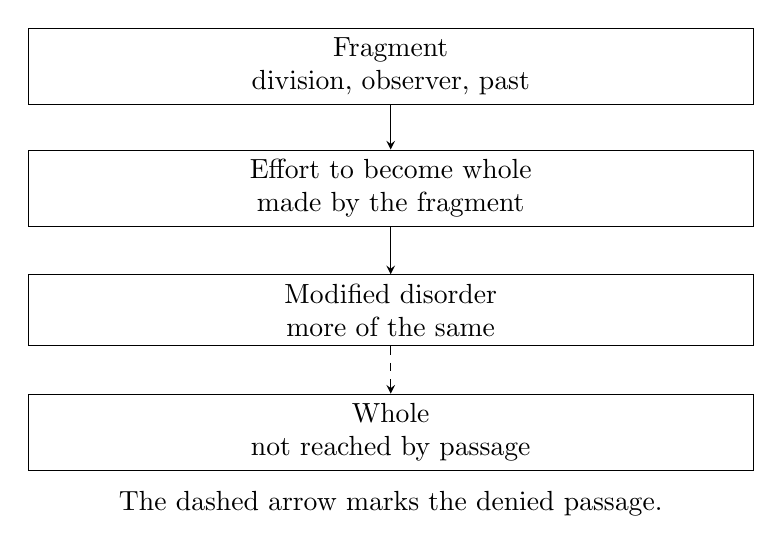
\begin{tikzpicture}[>=stealth]
\node[draw, align=center, text width=0.74\linewidth] (fragment) at (0,0) {Fragment\\division, observer, past};
\node[draw, align=center, text width=0.74\linewidth] (effort) at (0,-1.55) {Effort to become whole\\made by the fragment};
\node[draw, align=center, text width=0.74\linewidth] (modified) at (0,-3.10) {Modified disorder\\more of the same};
\node[draw, align=center, text width=0.74\linewidth] (whole) at (0,-4.65) {Whole\\not reached by passage};
\draw[->] (fragment) -- (effort);
\draw[->] (effort) -- (modified);
\draw[->, dashed] (modified) -- (whole);
\node[align=center, text width=0.70\linewidth] at (0,-5.55) {The dashed arrow marks the denied passage.};
\end{tikzpicture}
\caption{The fragment's attempt to become the whole remains a movement of fragmentation.}
\end{figure}

This is why the lecture refuses gradual progress inside disorder. Progress of that kind is proliferation, not transformation. The past may become more elaborate, but it remains the past.

\section{Listening, Regeneration, And Urgency}

The final movement asks whether a mind that has evolved in separation, contradiction, duality, and fragmentation can undergo regeneration. Krishnamurti is careful here. Regeneration is not produced by influence, propaganda, threat, punishment, or reward. If the mind changes because it expects reward, it has not changed.

The question returns to observation:
\begin{equation}
\mathrm{Observation\ by\ } O
\longrightarrow
\mathrm{Conflict}.
\end{equation}
The possible opening is stated cautiously:
\begin{equation}
\mathrm{Observation\ without\ } O
\longrightarrow
\mathrm{Regeneration}.
\end{equation}
This is not a method. The dialogue does not give exercises. It asks whether the fact of division can be observed without the observer. As long as an observer observes the fact, conflict continues.

At this point Krishnamurti turns to listening. The difficulty, he says, is that most people do not listen. If they do listen, they listen through conclusions. A communist listens up to a point; a mind already translating what it hears hears only its own distortion. Listening through conclusions is another continuation of the known:
\begin{equation}
\mathrm{Listening\ through\ Conclusions}
\longrightarrow
\mathrm{Continuation\ of\ the\ Known}.
\end{equation}
By contrast:
\begin{equation}
\mathrm{Listening\ itself}
\longrightarrow
\mathrm{Attention}.
\end{equation}

The examples at the end are not ornamental. Academic conferences where nobody listens, social talk that fills space, people moving from one novelty to another and calling it search, the house on fire: these are ways of restoring urgency. If the house is burning, one does not begin with secondary explanations. One acts.

The lecture closes by returning to relationship. When there is conflict in relationship, society furthers that conflict through education, national sovereignty, ideology, and the ordinary machinery of collective life. The serious question is therefore not abstract:
\begin{equation}
\mathrm{Relationship}
+
\mathrm{Freedom}
+
\mathrm{Knowledge}.
\end{equation}
These are not three separate topics. The question is whether functional knowledge can operate without becoming the observer in relationship, and whether relationship can be free of division.

\section{Summary}

The conversation begins with the observer and ends with attention. Its central discovery is that the observer is not outside the disorder it observes. The observer is the past: thought, memory, knowledge, image, hurt, hope, tradition, and conditioning. When such an observer enters relationship, division enters with it. Where there is division, conflict follows.

The chapter's compact structure is:
\begin{align}
\mathrm{Thought} &= \mathrm{Past},\\
O &= \mathrm{Past},\\
O &\longrightarrow \mathrm{Division},\\
\mathrm{Division} &\longrightarrow \mathrm{Conflict},\\
K_r &\longrightarrow \mathrm{No\ Actual\ Relationship}.
\end{align}
Against this, Krishnamurti does not reject knowledge. He distinguishes functional knowledge from knowledge as image in relationship. Knowledge is necessary for function; it becomes destructive when it acts as the observer between human beings.

The final pressure of the lecture is severe and exact. Freedom is not chaos. Freedom is order, order is virtue, and virtue is living action rather than reaction. The fragment cannot gradually become the whole, and disorder cannot transform itself by modification. What remains open for the continuing inquiry is whether there can be observation without the observer, and whether in such attention there is the beginning of regeneration.